\documentclass{beamer}

\usepackage[frenchb]{babel}
\usepackage[T1]{fontenc}
\usepackage[utf8]{inputenc}

\AtBeginSection[]
{
   \begin{frame}
       \frametitle{Outline}
       \tableofcontents[
       currentsubsection,
       sectionstyle=show/shaded,
       subsectionstyle=hide,
       ]
   \end{frame}
}

\usetheme{Rochester}
\setbeamertemplate{footline}[frame number]

\title[Short Paper Title]{Table de Hachage}
%\subtitle{Programmation Avancée}
\author{Vincent Aranega\\\texttt{vincent.aranega@univ-lille.fr}}
\date{\today}
\beamertemplatenavigationsymbolsempty{}

\begin{document}

  \maketitle

  \section{Pourquoi une nouvelle structure\@?}
  \begin{frame}{Temps d'accés aux éléments}
    Pour trouver la position d’un élément $e$ dans une structure de donnée de $n$ éléments :
    \begin{enumerate}
      \item{Liste : comparaison de la valeur des éléments de la liste
      avec \texttt{e}}
      \begin{itemize}
        \item{au pire : comparaison jusqu’au dernier élément}
        \item{recherche en \textit{O(n)}}
      \end{itemize}
      \item{Arbre : comparaison de la valeur des éléments de l’arbre avec $e$}
      \begin{itemize}
        \item{au pire : comparaison jusqu’à une feuille}
        \item{recherche en \textit{O(log (n))}}
      \end{itemize}
    \end{enumerate}

  $\rightarrow$ dépend du nombre d’éléments dans le TDA

  $\rightarrow$ si $n$ $\nearrow$ alors temps de la recherche $\nearrow$

  \end{frame}

  \begin{frame}{Dans l'idéal}
    Pour trouver la position d’un élément $e$ dans un ensemble de $n$ éléments :
    \begin{itemize}
      \item{accès direct à $e$}
      \item{un seul accès pour accéder à $e$}
      \item{recherche en \textit{O(1)}}
    \end{itemize}

    $\rightarrow$ ne dépend pas de nombre d’éléments $n$

    $\rightarrow$ $\forall$ $n$ temps de la recherche rapide

    $\rightarrow$ même si $n$ $\nearrow$ alors temps de la recherche = 1
  \end{frame}

  \section{Table à adressage direct}
  \subsection{Principe}
  \begin{frame}{Principe}
    \begin{itemize}
        \item{$U = \{0, 1, \ldots, m - 1\}$  est l'univers de tout les éléments/clés}
        \item{$K$ est un sous ensemble dynamique de $U$ représentant les clés effectivement cherchées/manipulées}
    \end{itemize}

    $\rightarrow$ Technique simple si l’univers des clés $U$ est petit

    \begin{itemize}
      \item{Représentation : table à adressage directe $T[0\ldots m - 1]$}
      \item{Chaque indice de $T$ correspond à une clé dans $U$}
      \item{2 éléments ne peuvent avoir la même clé}
    \end{itemize}


  \end{frame}

  \subsection{Exemple}
  \begin{frame}{Exemple}
    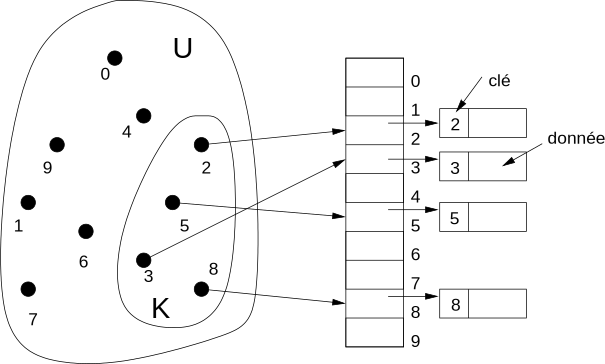
\includegraphics[width=\textwidth]{./imgs/direct}
  \end{frame}

  \subsection{Critiques}
  \begin{frame}{Problèmes}
    \begin{itemize}
      \item{Si $U$ est grand, $T$ ne tient pas en mémoire}
      \item{Si $|K| << |U|$ alors gaspillage de la mémoire}
    \end{itemize}
    $\rightarrow$ En pratique, quasi impossible à utiliser, solution à conserver
    lorsque $U$ est petit et $|K|$ est sensiblement égal à $|U|$
  \end{frame}

  %
  %
  % HASHTABLE
  %
  %

  \section{Table de hashage}
  \subsection{Principe}
  \begin{frame}{Principe}
    \begin{itemize}
      \item{la place d’un élément dans la table est calculée à partir de sa propre valeur}
      \item{calcul réalisé par une fonction de hachage : transforme la valeur de l’élément en une adresse dans un tableau}
      \item{recherche d’un élément : nombre constant de comparaisons \textit{O(1)}. Ne dépend pas du nombre d’éléments dans le tableau}
    \end{itemize}
  \end{frame}

  \subsection{Fonction de hachage}
  \begin{frame}{Fonction de hachage}
    \begin{itemize}
      \item{transforme la valeur d’un élément en position}
      \item{doit être facilement calculable (temps d’exécution de la fonction rapide sinon on perd le bénéfice de l’accès en \textit{O(1)})}
      \item{Pour une table $T$ et un élément $e$\\ $\exists$ une fonction de hachage $h$ telle que $T[h(e)] = e$ (si $e \in T$)}
    \end{itemize}

    \begin{block}{Attention}
      $h$ est une fonction déterministe sinon on ne pourrait
      pas retrouver nos données
    \end{block}
  \end{frame}

  \subsection{Exemple}
  \begin{frame}{Exemple}
    \begin{itemize}
      \item{Ensemble $K$}
      \begin{itemize}
        \item{Ensemble des éléments à stocker}
        \item{\{ serge, odile, luc, anne, annie,\\
        julie, basile, paula, marcel, elise \}}
      \end{itemize}
      \item{Table $T$ avec $n$}
      \begin{itemize}
        \item{taille de la table}
        \item{13}
      \end{itemize}
    \end{itemize}

    Rôle de la fonction de hachage $h$

    $\rightarrow$ associer à chaque élément e une position $h(e) \in [0..12]$
  \end{frame}

  \begin{frame}{Exemple}
    Exemple d’algorithme de fonction $h$ :
    \begin{enumerate}
      \item{Attribuer aux lettres $a,b,\ldots,z$ les valeurs $1,2,\ldots,26$}
      \item{$res = \sum$ valeurs des lettres de $e$}
      \item{$res = res\ +$ nombre de lettres de $e$}
      \item{$res = res\ mod(n)$ (ici $n = 13$)}
    \end{enumerate}
  \end{frame}
  \begin{frame}{Exemple}
    La position de l’élément $serge$ est donnée par $h(serge)$
    \begin{itemize}
      \item{$h(serge) = (54 + 5)mod13 = 7$}
      \item{$serge$ est à la position $7$ dans la table de hachage}
    \end{itemize}

    De même :
    \begin{itemize}
      \item{$h(odile) = (45 + 5)mod13 = 11$}
      \item{$h(luc) = (36 + 3)mod13 = 0$}
      \item{$h(anne) = (34 + 4)mod13 = 12$}
      \item{$h(annie) = (43 + 5)mod13 = 9$}
      \item{$h(jean) = 8, h(julie) = 10, h(basile) = 2$,\\
      $h(paule) = 4, h(elise) = 3, h(marcel) = 6$}
    \end{itemize}
  \end{frame}

  \begin{frame}{Exemple}
    \begin{table}[]
\centering
\begin{tabular}{r|c|}
\cline{2-2}
0  & Luc    \\ \cline{2-2}
1  &        \\ \cline{2-2}
2  & Basile \\ \cline{2-2}
3  & Elise                       \\ \cline{2-2}
4  & Paula                       \\ \cline{2-2}
5  &                             \\ \cline{2-2}
6  & Marcel                      \\ \cline{2-2}
7  & Serge                       \\ \cline{2-2}
8  & Jean                        \\ \cline{2-2}
9  & Annie                       \\ \cline{2-2}
10 & Julie                       \\ \cline{2-2}
11 & Odile                       \\ \cline{2-2}
12 & Anne                        \\ \cline{2-2}
\end{tabular}
\end{table}
  \end{frame}

  \begin{frame}{Exemple}
      serge ?
    \begin{table}[]
\centering
\begin{tabular}{r|c|}
\cline{2-2}
0  & luc    \\ \cline{2-2}
1  &        \\ \cline{2-2}
2  & basile \\ \cline{2-2}
3  & elise                       \\ \cline{2-2}
4  & paula                       \\ \cline{2-2}
5  &                             \\ \cline{2-2}
6  & marcel                      \\ \cline{2-2}
7  & serge                       \\ \cline{2-2}
8  & jean                        \\ \cline{2-2}
9  & annie                       \\ \cline{2-2}
10 & julie                       \\ \cline{2-2}
11 & odile                       \\ \cline{2-2}
12 & anne                        \\ \cline{2-2}
\end{tabular}
\end{table}

  \end{frame}

  \begin{frame}{Exemple}
    serge ? $\rightarrow$ $h(serge) = 7$
    \begin{table}[]
\centering
\begin{tabular}{r|c|}
\cline{2-2}
0  & luc    \\ \cline{2-2}
1  &        \\ \cline{2-2}
2  & basile \\ \cline{2-2}
3  & elise                       \\ \cline{2-2}
4  & paula                       \\ \cline{2-2}
5  &                             \\ \cline{2-2}
6  & marcel                      \\ \cline{2-2}
7  & serge                       \\ \cline{2-2}
8  & jean                        \\ \cline{2-2}
9  & annie                       \\ \cline{2-2}
10 & julie                       \\ \cline{2-2}
11 & odile                       \\ \cline{2-2}
12 & anne                        \\ \cline{2-2}
\end{tabular}
\end{table}
  \end{frame}

  \begin{frame}{Opération sur les tables de hachage}
    \begin{itemize}
      \item{\texttt{put(T, e)}}
      \begin{itemize}
        \item{insère une valeur $e$ dans la table $T$}
        \item{\texttt{T[h(e)] = e;}}
      \end{itemize}
      \item{\texttt{get(T, e)}}
      \begin{itemize}
        \item{retourne la valeur $e$ si elle est présente dans $T$, $NULL$ sinon (en considérant que chaque case du tableau à été init à $NULL$}
        \item{\texttt{return T[h(e)];}}
      \end{itemize}
      \item{\texttt{remove(T, e)}}
      \begin{itemize}
        \item{supprime l'entrée $e$ de la table $T$}
        \item{\texttt{T[h(e)] = NULL;}}
      \end{itemize}
    \end{itemize}
  \end{frame}

  \begin{frame}{Stockage d'informations complémentaires}
    \begin{itemize}
      \item{La clé sert à rechercher l'indice dans le tableau $T$}
      \item{Actuellement clé = valeur stockée}
      \item{Possible d'associer d'autres informations à la clé}
    \end{itemize}
    \centering
    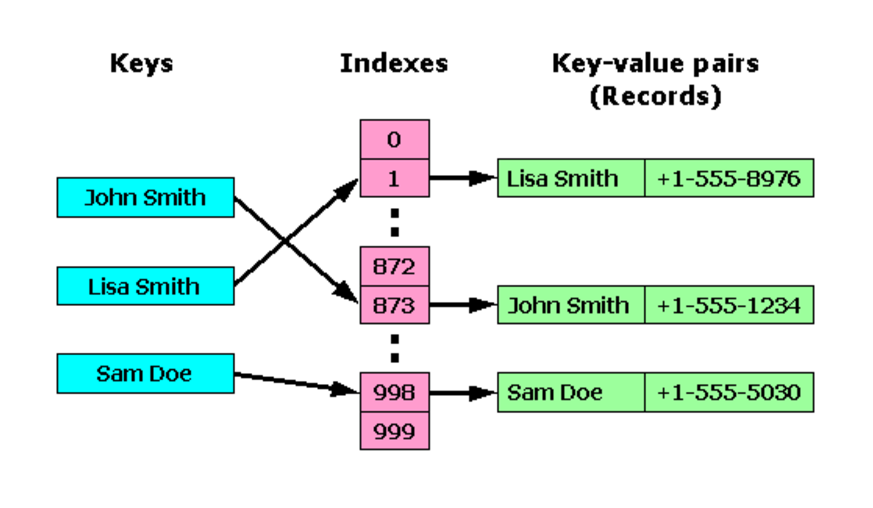
\includegraphics[scale=0.7]{./imgs/keyval.eps}
  \end{frame}

  \begin{frame}{Opération sur les tables de hachage}
    \begin{itemize}
      \item{On considère une structure \texttt{\{key, value\}} comme élément de la table}
      \item{\texttt{put(T, key, val)}}
      \begin{itemize}
        \item{insère un couple $key, val$ dans la table $T$}
        \item{\texttt{T[h(key)] = couple(key, val);}}
      \end{itemize}
      \item{\texttt{get(T, key)}}
      \begin{itemize}
        \item{retourne la valeur $val$ associée à $key$ si elle est présente dans $T$, $NULL$ sinon}
        \item{\texttt{return T[h(key)] != NULL ? T[h(key)].value : NULL;} (\texttt{T[h(key)]} retourne un couple)}
      \end{itemize}
      \item{\texttt{remove(T, key)}}
      \begin{itemize}
        \item{supprime l'entrée $key$ de la table $T$}
        \item{\texttt{T[h(key)] = NULL;}}
      \end{itemize}
    \end{itemize}
  \end{frame}

  \section{Collisions}

  \begin{frame}{Collision}

    Comme $|U| >> n$ ($n$ taille de $T$) $\rightarrow$ collision:
    \begin{itemize}
      \item{$\exists k, k' \in U\ |\ h(k) = h(k') \land k \ne k'$}
    \end{itemize}

    \begin{itemize}
      \item{Important de trouver la bonne fonction $h$}
      \item{$h$ est dépendant des valeurs à stocker}
    \end{itemize}

  \end{frame}

  \begin{frame}{Résolution}
    Diverses solutions:
    \begin{itemize}
      \item{Chaînage}
      \item{Adressage ouvert}
    \end{itemize}
    \begin{block}{Solution par chaînage}
      \begin{itemize}
        \item{Chaque valeur hachée est placée dans une liste}
        \item{La case $T[i]$ contient le pointeur vers la liste des éléments de clés $k$}
        \item{Si $T[i]$ ne désigne rien, alors il pointe sur $NULL$}
      \end{itemize}
    \end{block}
  \end{frame}

  \begin{frame}{Exemple}
    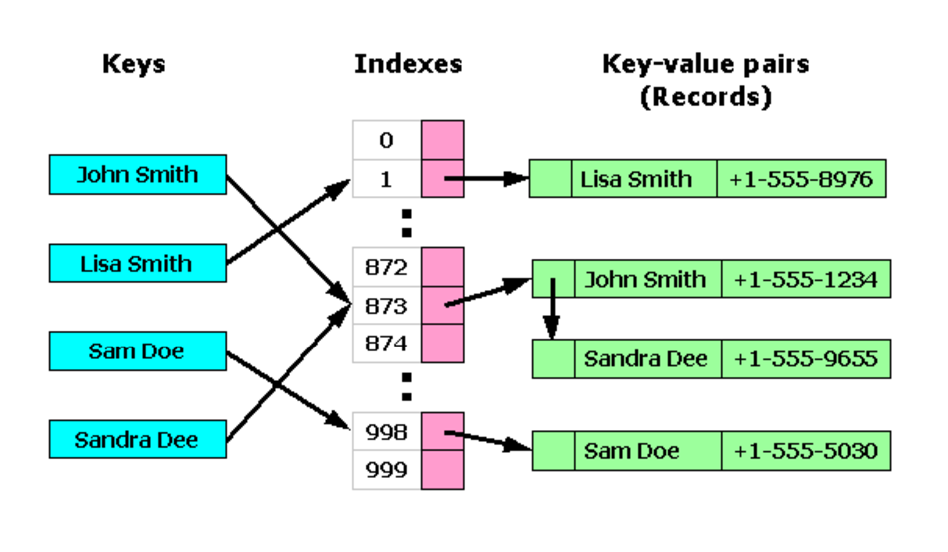
\includegraphics[scale=0.7]{./imgs/keyval2.eps}
  \end{frame}

  \begin{frame}{Opération sur les tables de hachage}
    \begin{itemize}
      \item{On considère une structure \texttt{\{key, value\}} comme élément de la liste contenue par chaque case de $T$}
      \item{\texttt{put(T, key, val)}}
      \begin{itemize}
        \item{on ajoute le couple $(key, val)$ en tête de la liste chaînée à la position $h(k)$ du tableau}
        \item{\texttt{ajout\_tete(T[h(key)], couple(key, val));}}
      \end{itemize}
      \item{\texttt{get(T, key)}}
      \begin{itemize}
        \item{on cherche la $key$ dans la liste située à $h(key)$ (recherche dans liste de couple)}
        \item{\texttt{couple = list\_find(T[h(key)], key); \\
                      return couple != NULL ? couple.value : NULL;}}
      \end{itemize}
      \item{\texttt{remove(T, key)}}
      \begin{itemize}
        \item{on supprime le couple $(key, val)$ situé de la liste contenue en $h(key)$}
        \item{\texttt{supp(T[h(key)], key);}}
      \end{itemize}
    \end{itemize}
  \end{frame}

  %\section{Méthode de hachage}
  \begin{frame}{Conclusion}
    \begin{itemize}
      \item{Ajout d'informations et recherche efficace}
      \item{Association clé, valeur}
      \item{Valeurs ordonnable ou non (pas obligatoire)}
      \item{Dépendant d'une fonction de hachage}
      \item{Difficulté $\rightarrow$ déterminer fonction de hachage}
    \end{itemize}
  \end{frame}

  \begin{frame}{Comparaison}
    \begin{table}[]
\centering
\begin{tabular}{cccc}
\multicolumn{1}{l}{}                   & \multicolumn{3}{c}{Moyenne}                                                                     \\
\multicolumn{1}{l|}{}                  & \multicolumn{1}{l}{recherche} & \multicolumn{1}{l}{insertion} & \multicolumn{1}{l}{suppression} \\ \hline
\multicolumn{1}{c|}{liste}             & \textit{O(n)}                 & \textit{O(1)}                 & \textit{O(n)}                   \\
\multicolumn{1}{c|}{arbres binaires}   & \textit{O(log n)}             & \textit{O(log n)}             & \textit{O(log n)}               \\
\multicolumn{1}{c|}{tables de hachage} & \textit{O(1)}                 & \textit{O(1)}                 & \textit{O(1)}
\end{tabular}
\end{table}

\begin{table}[]
\centering
\begin{tabular}{cccc}
\multicolumn{1}{l}{}                   & \multicolumn{3}{c}{Pire cas}                                                                    \\
\multicolumn{1}{l|}{}                  & \multicolumn{1}{l}{recherche} & \multicolumn{1}{l}{insertion} & \multicolumn{1}{l}{suppression} \\ \hline
\multicolumn{1}{c|}{liste}             & \textit{O(n)}                 & \textit{O(1)}                 & \textit{O(n)}                   \\
\multicolumn{1}{c|}{arbres binaires}   & \textit{O(n)}                 & \textit{O(n)}                 & \textit{O(n)}                   \\
\multicolumn{1}{c|}{tables de hachage} & \textit{O(n)}                 & \textit{O(1)}                 & \textit{O(n)}
\end{tabular}
\end{table}
  \end{frame}

  \begin{frame}{Références}
    \begin{itemize}
      \item{Algorithme et Structure de données -- Jean-Charles Régin}
      \item{Les tables de hachage -- Christophe Gonzales, Pierre-Henri Wuillemin}
      \item{Tables de hachage -- ENSIEE}
      \item{Table de hachage -- B. Jacob}
      \item{Les Tables de Hachage -- Jean-March Nicod}
    \end{itemize}
  \end{frame}

\end{document}
